\chapter{}\label{chp:4}

Consider the graph shown in \Cref{fig:8}, each node representing a Wireless Sensor Node. The chosen communication protocol requires unique frequency channels in each 2-hop neighborhood.

a) Suppose 9 channels are available, can the chosen communication protocol be used in the shown network?
(yes, a.smt)

b) Determine the minimum number of channels required to be able to use the chosen communication protocol in the shown network.
(7, b2.smt (6) => UNSAT, b1.smt (7) => SAT)

c) Suppose a different communication protocol requires unique frequency channels in each 3-hop neighborhood instead and 11 channels are available. Determine if this other communication protocol can be used in the shown network.
(yes, c.smt)

\begin{figure}[H]
    \centering
    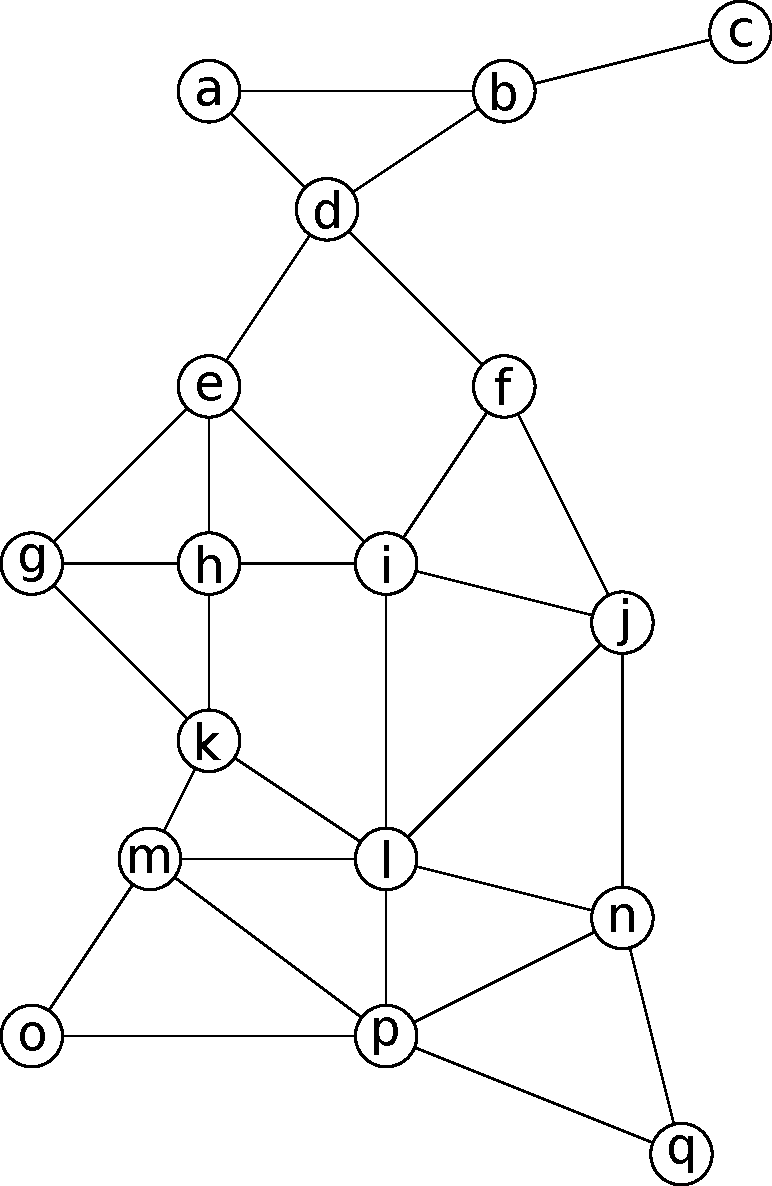
\includegraphics[width=\columnwidth]{8/graph.pdf}
    \caption{The graph depicting the connectedness of the Wireless Sensor Network under consideration.}
    \label{fig:8}
\end{figure}
